In order to evaluate our proposal, we ran experiments over three standard corpora, namely: 20 News Groups\footnote{http://...}, NIPS 2012\footnote{http://...} and Reuters50\footnote{http://...}. Table~\ref{tab:stats} summarizes the characteristics of the these corpora. Each corpus is divided in a training and test set with a ratio 80-20 percent. Models are evaluated according to their perplexity on the test set and we follow here the  approach of \cite{asuncion_smoothing_2009} based on the following fold-in procedure: the word-topic distribution is learned on the training set and considered fixed, whereas the document-topic distribution is learned for each document of the test set, by using the first half of the document only; the perplexity is then computed on each test document, then averaged over all test documents, using:
%
\[
\begin{array}{l@{\hspace{.3cm}}l}
\log p(x^{test}) = \sum_{dw} n_{dw} \log \sum_k \hat{\theta}_{kd} \hat{\phi}_{wk} \\
perplexity(x^{test}) = \exp(- \frac{\log p(x^{test})}{\sum_d n_d})
\end{array}
\]
%
with $n_d = \sum_w n_{dw}$.

We have compared several variants of the LDA model according to the previous development:
%
\begin{itemize}
\item With a symmetric prior, fixed or estimated with the EM type 2 procedure, for $\alpha$ and/or $\beta$;
\item With a fixed asymmetric prior, for $\alpha$ and/or $\beta$;
\item With a Boojum prior, estimated with the procedure described in Section~\ref{sec:LDAwithPrior}, for $\alpha$ and/or $\beta$.
\end{itemize}
%
The best combination is obtained with a fixed asymmetric prior on $\alpha$ and a Boojum on $\beta$. In the remainder, we refer to this model as {\it conjugate LDA} ({\it ldaconjugate} for short). Both the Boojum prior and the asymmetric prior on $\alpha$ yield better results than the symmetric one, in acordance with the results obtained in \cite{wallach_rethinking_2009} which illustrate the imporatnce of an asymmetric prior on the document-topic distribution. Furthermore, the Boojum prior on $\beta$ helps here to improve the models.

Figure~\ref{fig:1} illustrates the behavior of the conjugate LDA model wrt to the standard LDA model (with symmetric priors estimated via the EM type 2 procedure). The perplexity is averaged over 10 runs to assess the influence of the random initilization of the parameters. The number of topics is set to 6 and the number of documents to 1000. As one can note, the perplexity of the conjugate model is lower than the one of the standard model, and decreases with the number of iterations, as expected.

Figure~\ref{fig:2} shows how the conjugate LDA model behaves, compared to the standard LDA model, with respect to the size of the collection. Here again, the number of topics $K$ is set to 6. As one can note, the ratio of perplexity is below 1 when the size of the collections is small (roughly below 3000 documents), and above 1 after that. This indicates that the conjugate LDA model compares favorably to the standard model for small collections, which can be explained by the additional information brought by the prior on such collections (the influence of the prior then decreases with the size of the collection). For higher values of $K$, a similar tendency is obtained, but the difference between the models vanishes for $K \ge 30$ in our experiments.

Figure~\ref{fig:3} ilsutrates the impact of the Boojum prior on the word-topic distribution. ???

Lastly, Figure~\ref{fig:time} compares the execution time of the inference procedures for the two models for $K=20$. Similar plots are obtained for different values of $K$. As one can note, there is no significant difference between the inference in the conjugate and the standard models.

\begin{figure}[h]
\label{fig:pp_D}
%\vspace{.3in}
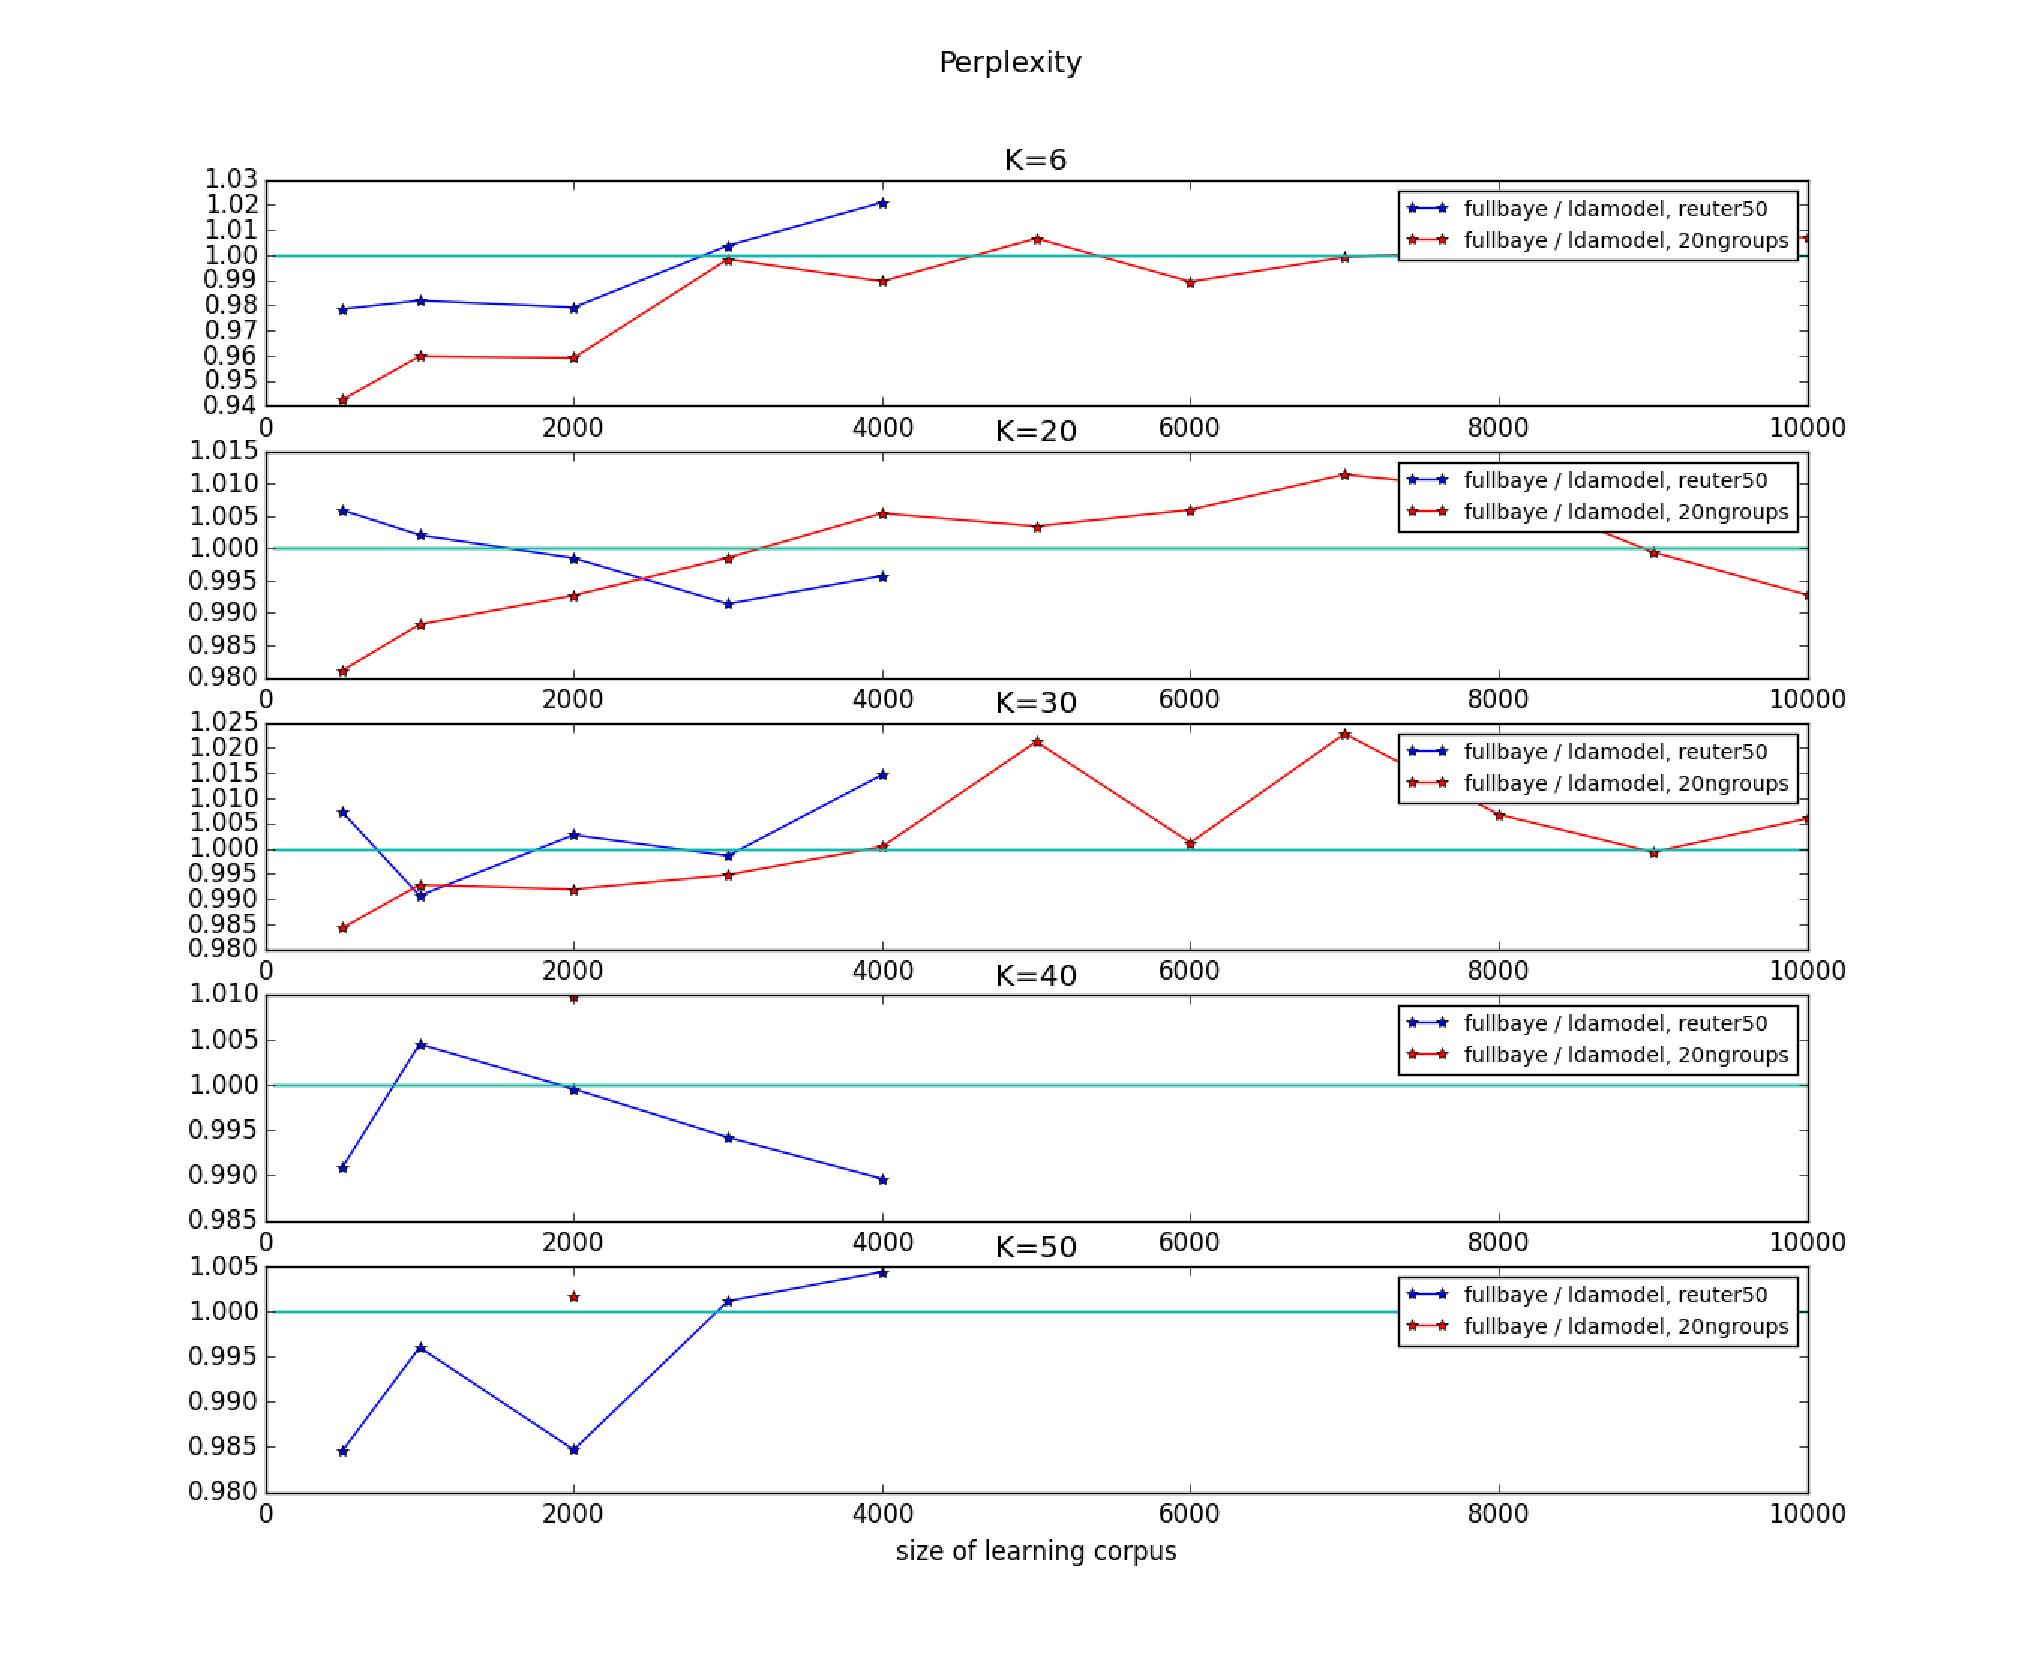
\includegraphics[width=9cm, height=14cm]{results/pp_D}
%\vspace{.3in}
\caption{Ratio of perplexity of the conjugate LDA model over the standard LDA model on several size of dataset and for different number of topic}
\end{figure}

\begin{figure}[h]
\label{fig:pp_conv}
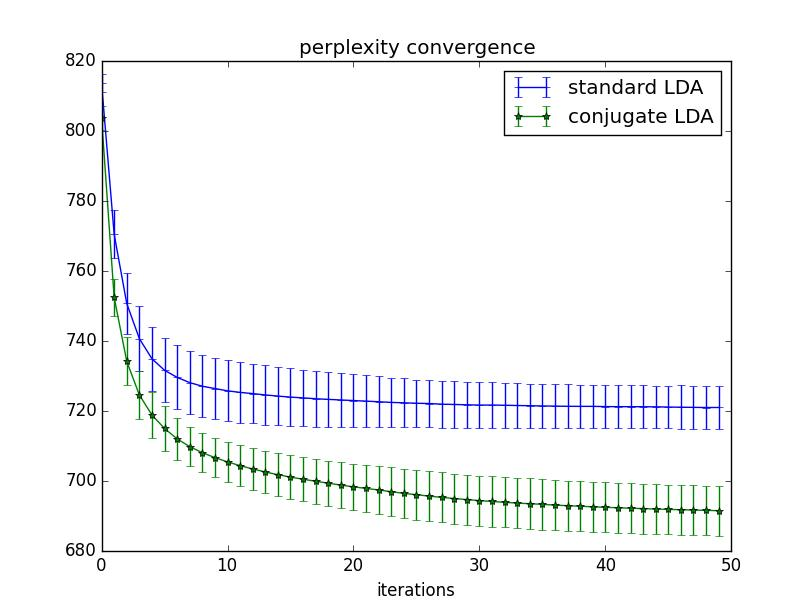
\includegraphics[scale=0.4]{results/pp_conv}
\caption{Result of perplecity on testing set at each iterations of the variationnal bayes iteratino for the 20 news group corpus}
\end{figure}

\begin{figure}[h]
\label{fig:time}
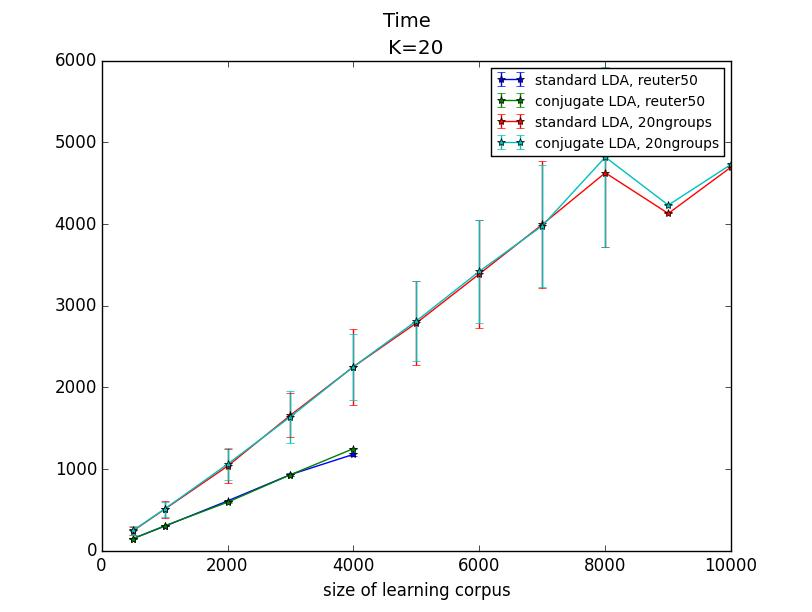
\includegraphics[scale=0.4]{results/time}
\caption{Time of inference for 50 iterations of variational bayes.}
\end{figure}

\begin{figure}[h]
\label{fig:pp_K}
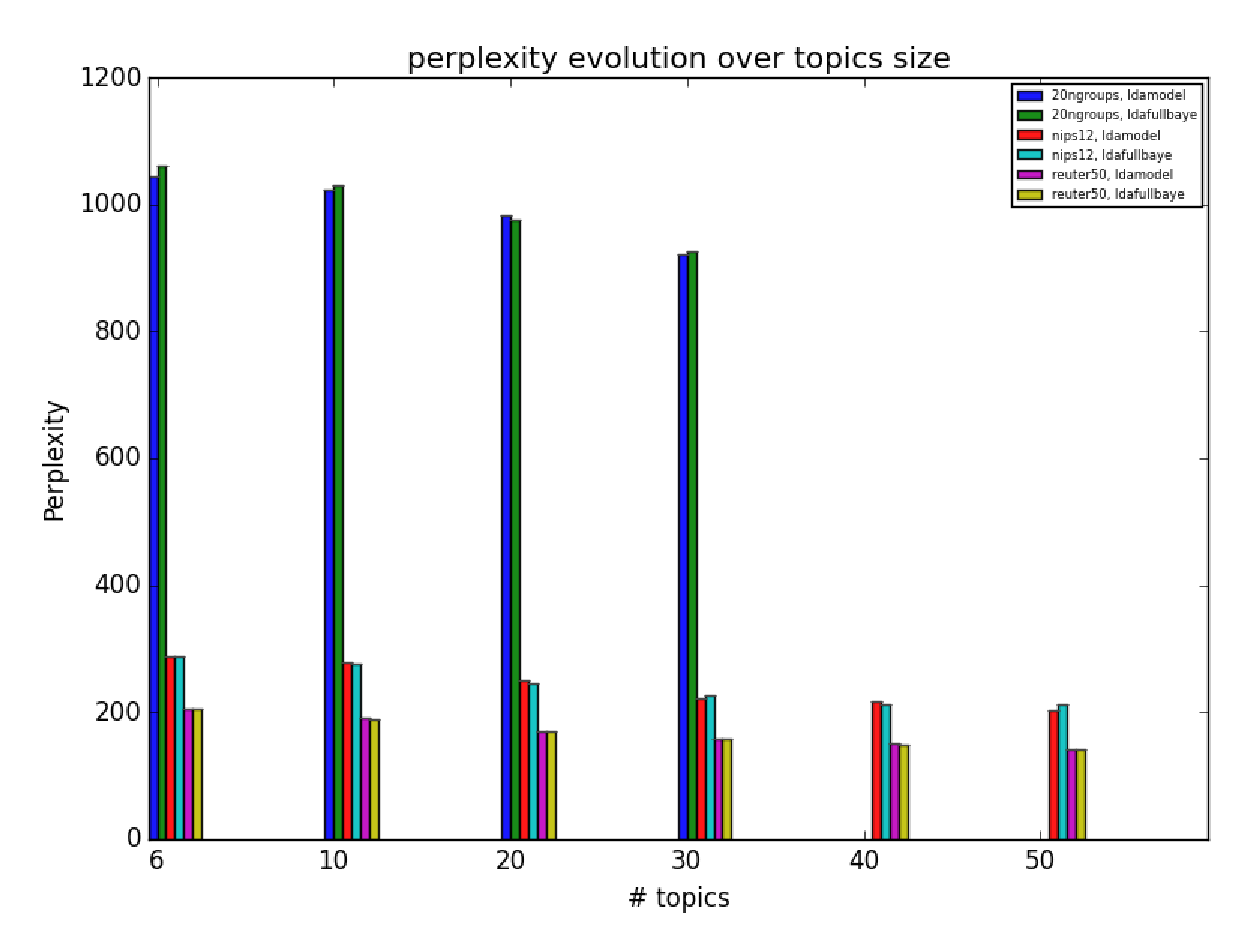
\includegraphics[scale=0.4]{results/pp_K}
\caption{For several number of topic, we show the perplexity of all the corpus for the classical LDA and the boojum extension.}
\end{figure}

%Each inference procedure was run over 50 iterations and reproduced 10 times to provide a stability measure. Therefore, the figure shows the mean perplexity for each run and his variance.
